\documentclass[a6paper, 11pt, parskip=half, DIV=15]{scrartcl}

\usepackage[dvipsnames]{xcolor}
\usepackage{tikz}

\usepackage{ragged2e}
% Minimize unwanted hyphenation
\tolerance=1
\emergencystretch=\maxdimen
\hyphenpenalty=1
\hbadness=10000

\usepackage{fontspec}

\setkomafont{section}{\setmainfont{Dakota Rough}\LARGE}
\setkomafont{subsection}{\setmainfont{Dakota Rough}\Large\lowercase}
\setkomafont{subsubsection}{\setmainfont{Dakota Rough}\large\lowercase}

% Adjust spacing before and after section headings
\RedeclareSectionCommand[
  runin=false,
  beforeskip=1.0\baselineskip,
  afterskip=-0.25\baselineskip
]{section}

% Adjust spacing before and after subsection headings
\RedeclareSectionCommand[
  runin=false,
  beforeskip=1.0\baselineskip,
  afterskip=-0.25\baselineskip
]{subsection}

% Adjust spacing before and after subsubsection headings
\RedeclareSectionCommand[
  runin=false,
  beforeskip=1.0\baselineskip,
  afterskip=-0.25\baselineskip
]{subsubsection}


\usepackage{enumitem}
\setlist[description]{labelindent=0pt, labelsep=\widthof{ }, leftmargin=\widthof{\textbf{License: }}, font=\setmainfont{URWClassico}\bfseries}

\usepackage{hyperref}
\usepackage[type={CC}, version={4.0}, modifier={by-sa}]{doclicense} % Add text and icons for creative commons license
%\usepackage{array}

\raggedright
\pagestyle{empty}
\begin{document}

\begin{titlepage}
\enlargethispage{3.0\baselineskip}
%\setmainfont[Scale=2.1]{DarkCrystal-Outline}
\setmainfont[Scale=1.55]{Dakota Rough}
\Huge
\begin{center}
\vspace*{-0.5\baselineskip}
Not\ \ From\\[1ex]
Around\ \ Here

\vfill
\begin{tikzpicture}
\node[draw, line width=0.25cm, rotate=7.5, inner sep=1pt] at (0,0) {
\includegraphics[scale=0.47]{Images/alien_beach_vacation.png}};
\end{tikzpicture}
\vfill
\huge
%\setmainfont{Cochin}
\setmainfont{Caveat}
A Socratic Worldbuilding Game\\
by Michael Purcell
\end{center}
\end{titlepage}
\thispagestyle{empty}
\enlargethispage{1.75\baselineskip}
\setmainfont{Special Elite}
\normalsize
\noindent ATTN: All R.H. Employees

Recently, an increasing proportion of our guests have been aliens. While we have managed to accommodate them on an ad hoc basis so far, we need to establish some official policies to ensure that all of our guests continue to receive our signature brand of world-class service. 

To that end, I will be hosting mandatory meeting tomorrow evening to discuss the matter.
The following topics are of particular interest:
\begin{enumerate}[nosep]
	\item Dining and Entertainment
	\item Guest Safety and Comfort
	\item Payment and Gratuities
	\item Reputation and Marketing
\end{enumerate}   

Please familiarize yourself with a few aspects of the aliens' biology, history, and culture ahead of time.
By sharing our expertise, we can all learn a bit more about our new guests and find new ways make them feel welcome them here.

\hspace{4.5cm}\huge\setmainfont{Caveat}- Arthur B.
\setmainfont{Quicksand}
\normalsize

\newpage
\enlargethispage{1.75\baselineskip}

\section*{Overview}
This is a worldbuilding game. It is intended for groups of three to six players and can be played in about one hour.

You will assume the roles of hospitality workers at a tropical resort. Recently, your clientele has started to include an increasing number of extraterrestrial aliens. The general manager has called a meeting to discuss the situation.

\vfill

\begin{center}
\begin{tikzpicture}
\node[draw, inner sep=1pt, line width=0.15cm, rotate=-4] at (0,0) {
\includegraphics[scale=0.55]{Images/alien_drinking.png}};
\end{tikzpicture}
\end{center}

\vfill

You will ask and answer a series of questions about your alien guests and how they will affect life at the resort. By doing so, you will describe the world your characters inhabit.

\newpage
\enlargethispage{1.75\baselineskip}

\section*{Characters}
You will portray a hospitality worker who is employed at an all-inclusive tropical resort. To create your character,
\begin{enumerate}[nosep]
	\item Describe what you do at the resort.
	\item Describe your mannerisms and physical appearance.
	\item Describe two types of questions about the extra terrestrials that you can answer.
	\item Describe one objective that you want to accomplish at the meeting.
\end{enumerate}
Introduce yourself to the other characters before the meeting begins.

\section*{Gameplay}
The game takes place over five rounds. 
During each of the first four rounds, you will discuss one topic that the general manager has identified as being of particular interest.
During the last round, you will discuss how to respond to the issues raised in previous rounds. 

\newpage
\enlargethispage{1.75\baselineskip}

\subsection*{Topics}
The general manager has identified four topics of particular interest for discussion:
\begin{enumerate}[nosep]
	\item Dining and Entertainment
	\item Guest Safety and Comfort
	\item Payment and Gratuities
	\item Reputation and Marketing
\end{enumerate}
In each of the first four rounds, you will discuss one of these topics.

\subsection*{Facilitators}
One player should act as the facilitator in each round. Their job is to ensure that everyone has a chance to contribute and that the discussion stays focused on the topic at hand.

\subsection*{Questions}
During the game, you will ask and answer questions about the extraterrestrials and the game's setting.
You will invent the answers to these questions as they arise to describe the world that your characters inhabit.

\newpage
\enlargethispage{1.75\baselineskip}


\subsubsection*{Factual Questions}

Factual questions are questions about the nature of some part of the game's setting.
These questions are usually stated using one of the standard interrogatives: who, what, where, when, why, and how.

\vfill

\begin{center}
\begin{tikzpicture}
\node[draw, inner sep=1pt, line width=0.2cm, rotate=10] at (0,0) {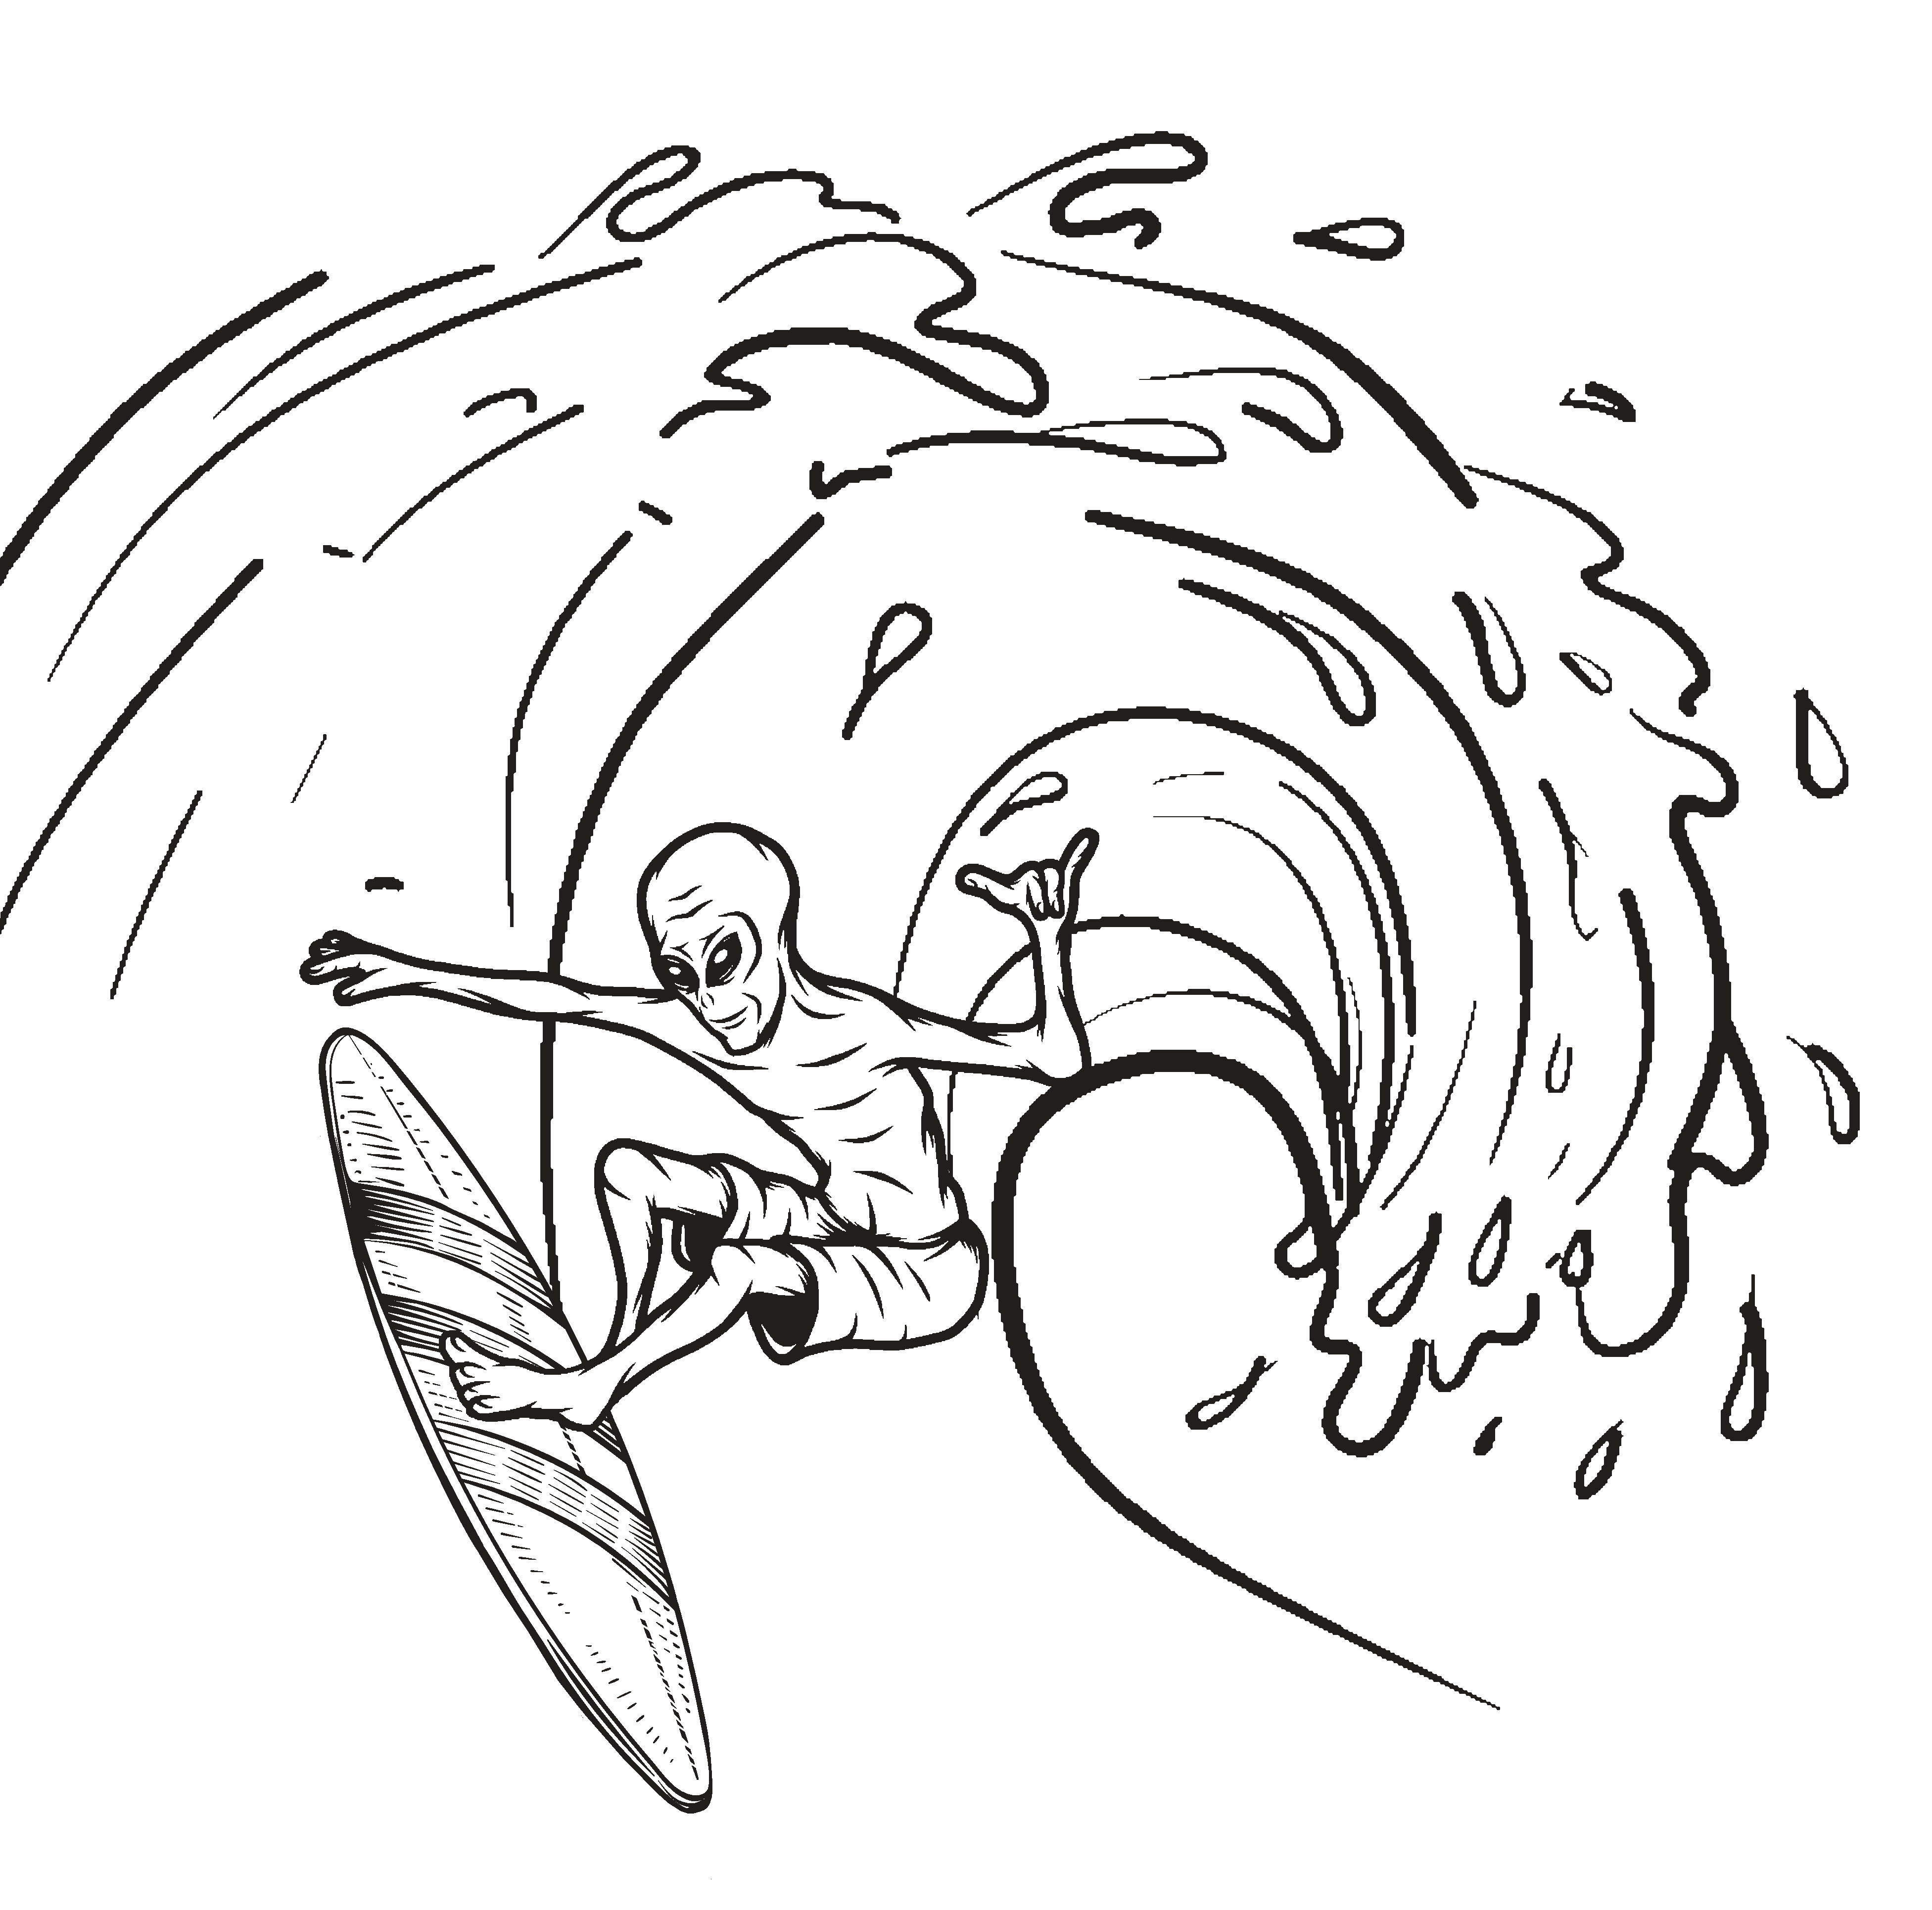
\includegraphics[scale=0.0475]{Images/alien_surfing.png}};
\end{tikzpicture}
\end{center}

\vfill

Whoever is best suited to answer each factual question should do so.
Your answers should be consistent with any details about the setting that have been previously established.
Beyond that, however, you are free to invent any details you like as a part of your answers.

\newpage
\enlargethispage{1.75\baselineskip}

\subsubsection*{Socratic Questions}
Socratic questions are questions that encourage critical thinking.
These questions frequently arise as follow-up questions after a player establishes a new detail about the game's setting.

Socratic questions are often intended to do one or more of the following:
\begin{itemize}[nosep]
	\item Clarify concepts
	\item Challenge assumptions
	\item Probe evidence
	\item Discover alternative viewpoints
	\item Explore implications
\end{itemize}

After someone answers a factual question, you should use Socratic questions to help them flesh out their answer and explain how any new details they introduced interact with other details that had been previously established.

\vfill

\hrulefill
\begin{description}[nosep]
\item[\textbf{Contact}:] \href{mailto:nfah.ttrpg@gmail.com}{nfah.ttrpg@gmail.com}\\
\item[\textbf{License}:] \doclicenseText%This work is licensed under a ``CC BY 4.0'' license.
\end{description}

\newpage
\enlargethispage{1.75\baselineskip}

\subsection*{Action Items}
During the last round, your job is to decide what you are going to do next.
You should describe what you think needs to be done, what you can do yourselves, and what you need help with.

\vfill

\begin{center}
\begin{tikzpicture}
\node[draw, inner sep=1pt, line width=0.2cm, rotate=-4] at (0,0) {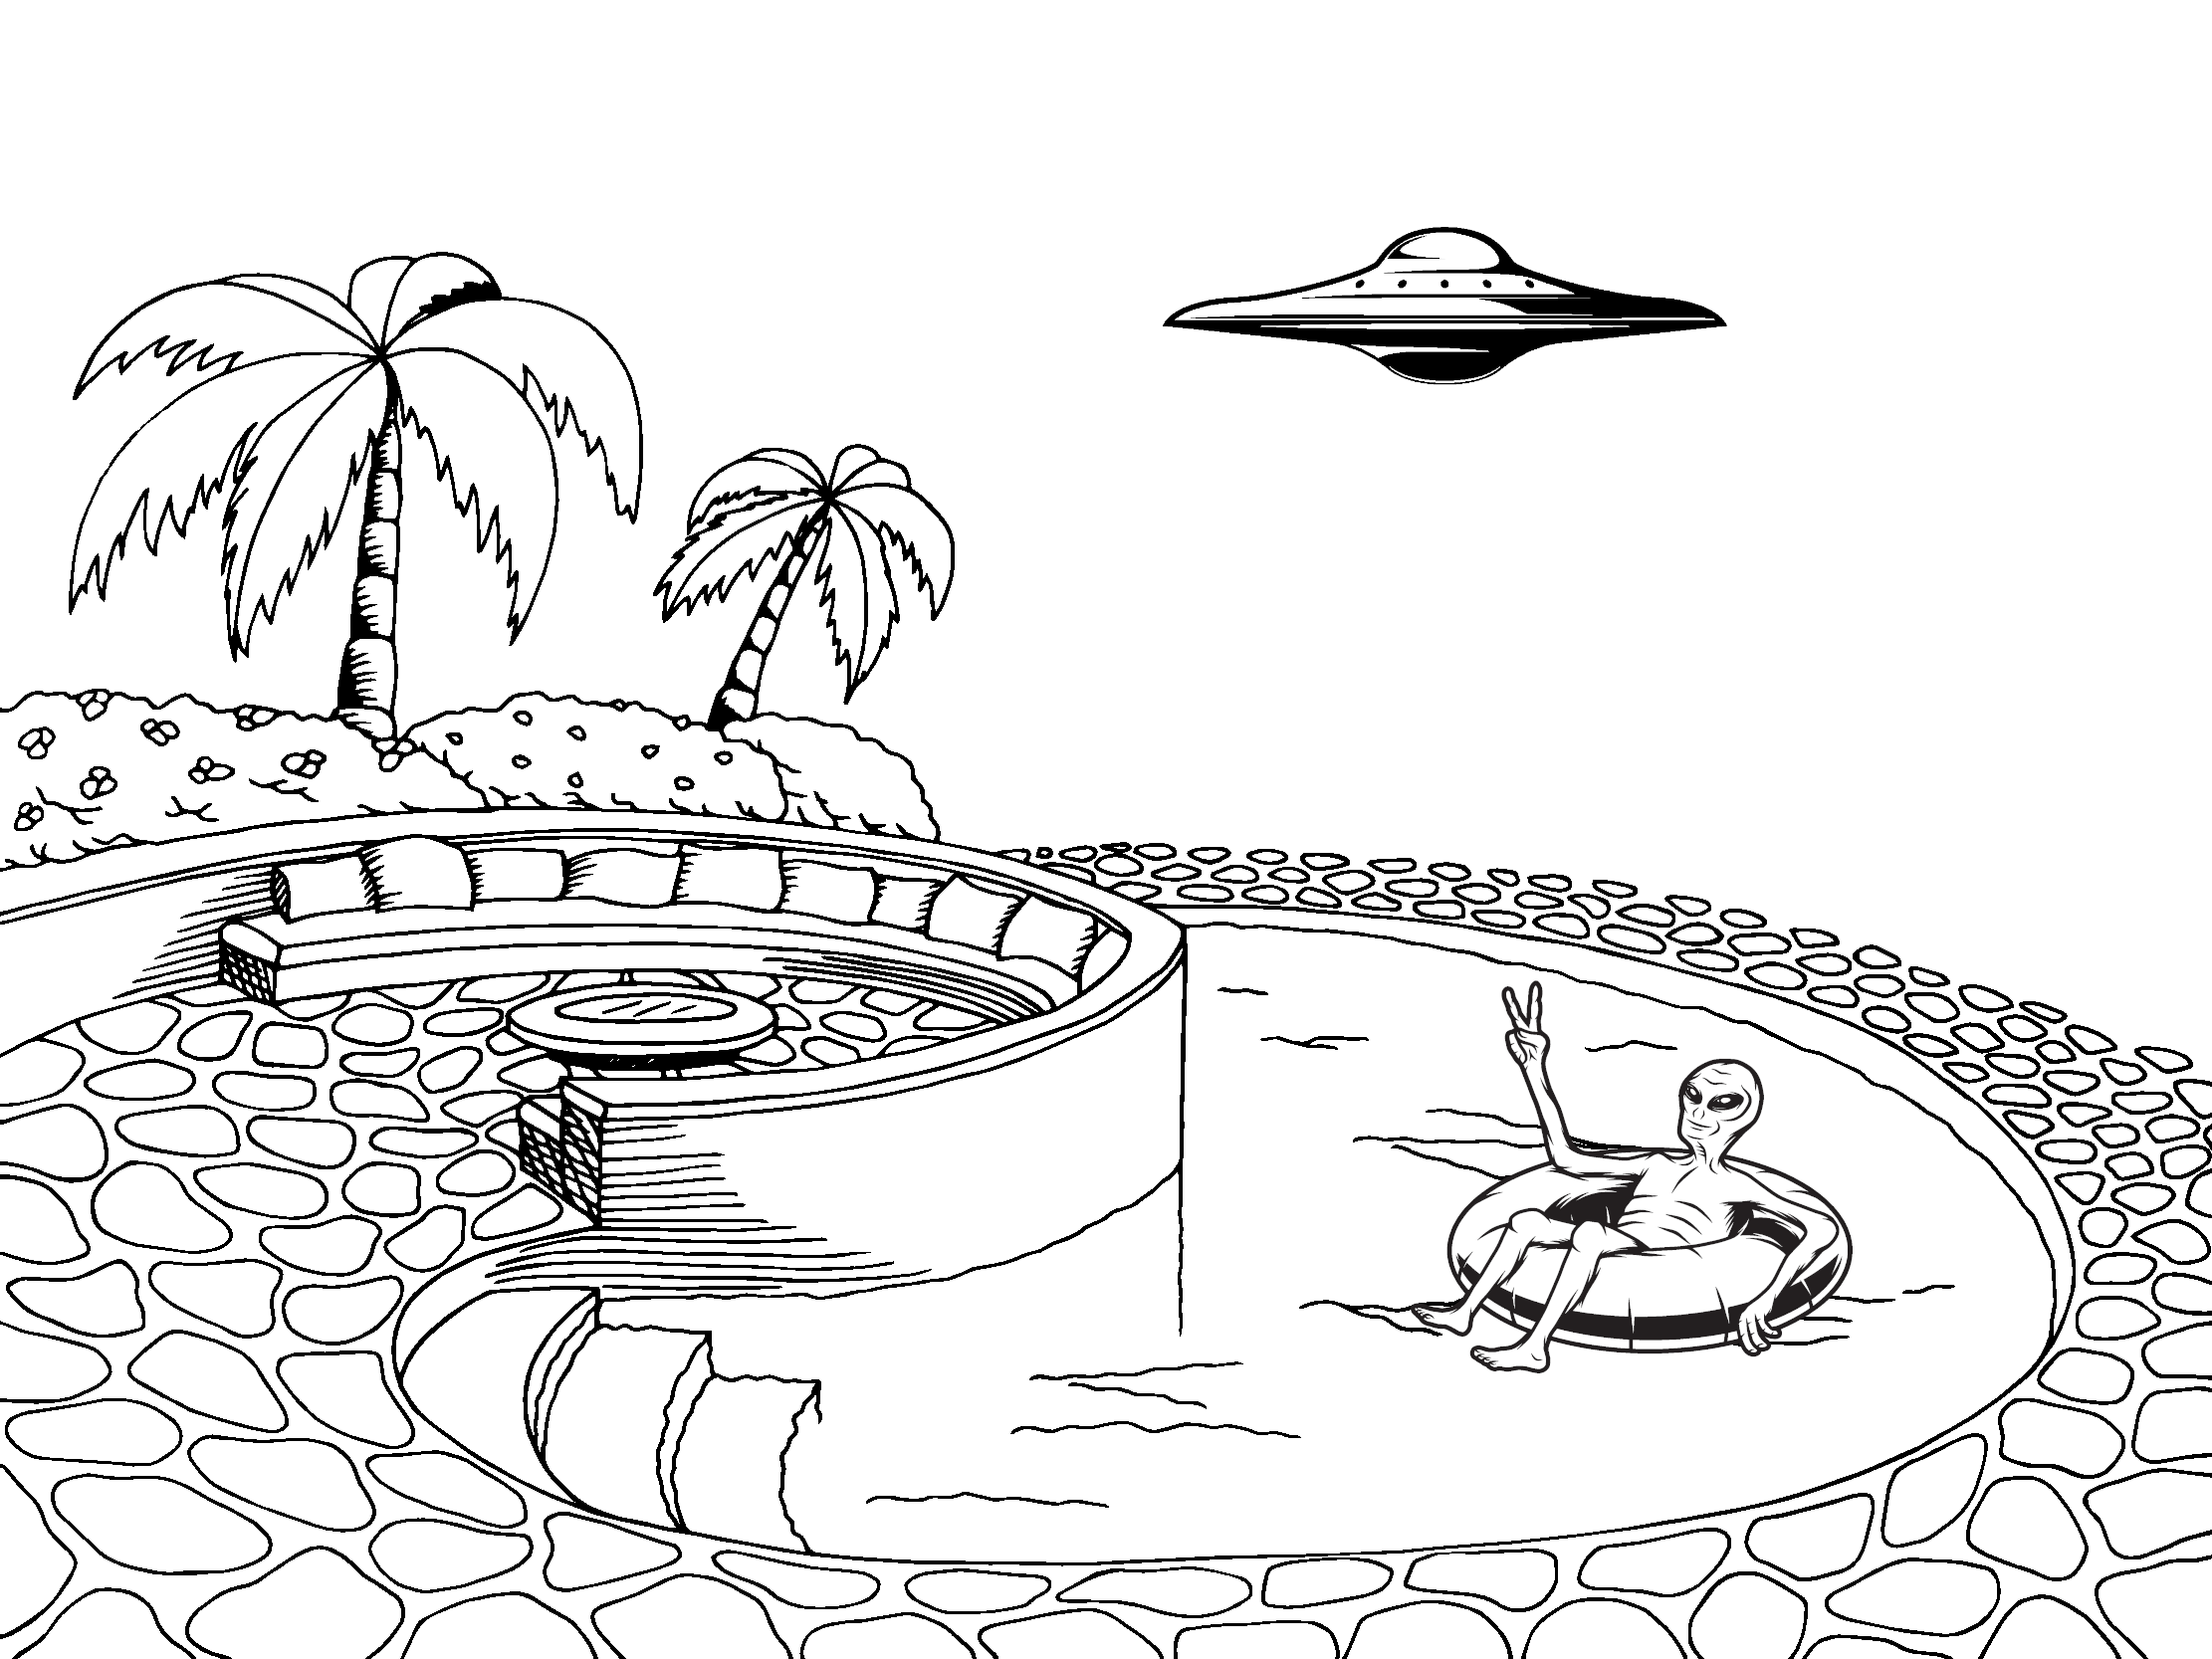
\includegraphics[scale=0.1]{Images/alien_pool.png}};
\end{tikzpicture}
\end{center}

\vfill

As in the previous rounds, you should use Socratic questions to help each other understand what you are proposing and why you think that your proposal describes a reasonable course of action.
\end{document}